% This file was converted from HTML to LaTeX with
% gnuhtml2latex program
% (c) Tomasz Wegrzanowski <maniek@beer.com> 1999
% (c) Gunnar Wolf <gwolf@gwolf.org> 2005-2010
% Version : 0.4.
\section{Datenstrukturen}
\subsection{To Do}
\begin{itemize}
\item  zu Linien:
\begin{itemize}
	\item  Was passiert, wenn ein Endpunkt nicht sichtbar ist? Bekommen wir einen Punkt am Rand des Sichtfeldes? Vektor...?
	\item  Wir bekommen \textit{\textbf{nicht}} die Info, \textit{\textbf{welche Linie}}
 das ist, wenn wir eine sehen. Wenn wir Linien als statische Objekte für
 unsere Schablone nutzen wollen, müssen wir das selbst rausfinden. Dazu 
zwei Möglichkeiten:
	\begin{itemize}
		\item  Wir verlassen uns darauf, dass wir immer zusätzlich noch Flags oder Goalpoles sehen und es daraus ableiten können.
		\item  Bei genügender Confidency über die eigene Position, könnten wir auch diese Information dazu nutzen.
	\end{itemize}
\end{itemize}
\item Gewichtung
\end{itemize}
\subsection{Weltenmodell }
Umgesetzt in der world.py\\
Ziel ist es das Spielfeld intern darzustellen und mit möglichst 
vielen und genauen Daten zu füllen die dem Agenten später als Grundlage 
für seine Entscheidungen dienen.
Um die Kommunikation zwischen den Naos zu erleichtern haben wir uns für 
ein statisches Weltbild entschieden. Konkret heißt das, dass wir den 
Koordinatenursprung im Spielmittelfeld angesiedelt haben und nicht an 
der Position des Agenten. Dadurch erhalten wir feste Positionen für 
unsere sogenannten static entities wie die Flagen, Linien und 
Torpfosten. (Fest meint hier während eines Spiels, die Spielfeldgröße, 
die sich im Laufe der Entwicklung öfters geändert hat, kann dem 
Konstruktor der world übergeben werden.)\\
Das Spielfeld sieht wir folgt aus:\\
\begin{figure}[h]
\begin{center}
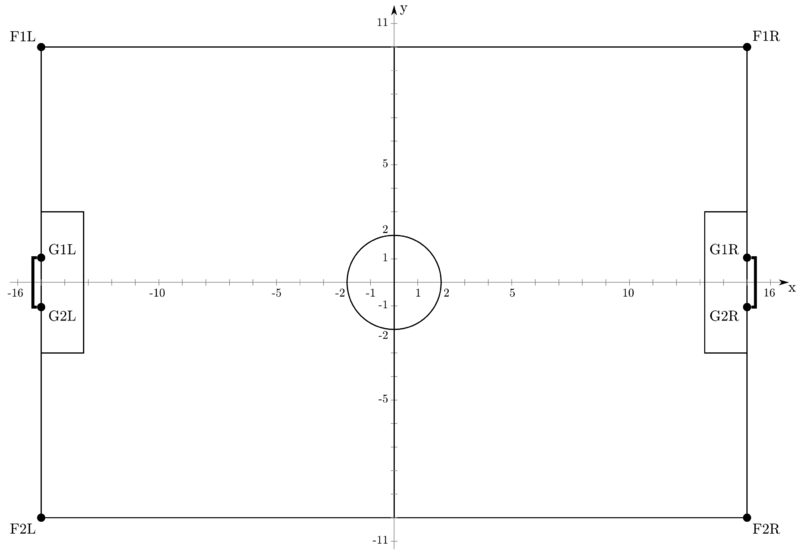
\includegraphics[scale=2.6]{800px-SoccerSimulation_FieldPlan}
\end{center}
\caption{Spielfeldmaße}
\end{figure}
\\
Wichtig dabei zu beachten ist das sowohl die 4 Eckfahnen als auch
 die 4 Torpfosten eindeutige Namen in der Simulation haben und auch vom 
Nao unterschieden werden können.\\
Dazu kommen dann noch bewegliche Objekte (die mobile entities) 
wie andere Mitspieler und der Ball, deren aktuelle Position permanent 
neu berechnet werden müssen. Dazu erhalten wir alle 3 Zyklen von der 
"virtuellen Kamera" des Naos was dieser gerade sieht. Die Daten werden 
von der \textit{perception.py} verarbeitet und von ihr in die world bzw. die nao Klasse geschrieben.

\subsection{Nao}
Umgesetzt in der nao.py\\
Die nao.py hat das Ziel alle Agenten spezifischen Daten zu 
sammeln. Dazu gehören die eigenen Gelenkstellungen, die momentane 
Aufgabe, die Aktuelle Lage (also aufrecht, auf dem Rücken ect.)

\subsection{Klassenmodell des Gegenstandsbereiches}
(Stand 09.06)\\
\begin{figure}[h]
\begin{center}
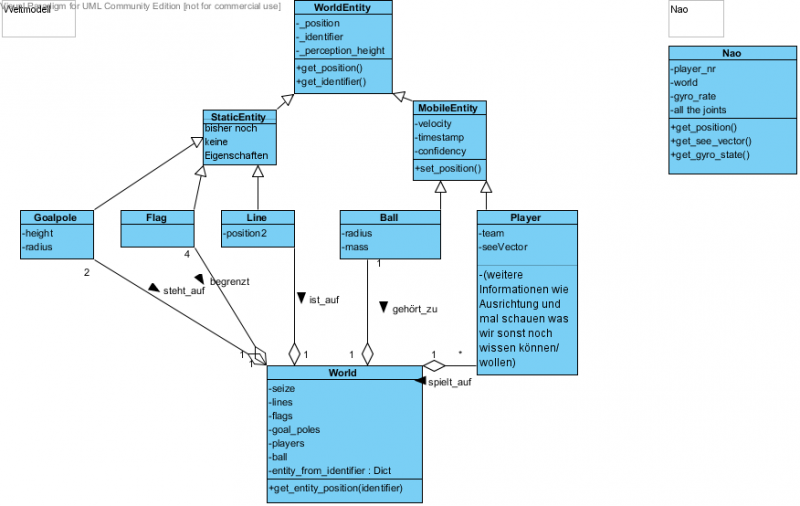
\includegraphics[scale=0.6]{800px-Weltenmodell}
\end{center}
\caption{Klassenmodell des Gegenstandsbereichs}
\end{figure}


\subsection{Perception}
Umgesetzt in perception.py -Hier passiert die  ganze Magie~:D

\subsubsection{Distanzberechnung: 3D-Kugelkoordinaten zu 2D kartesischen}
\begin{figure}[h]
\begin{center}
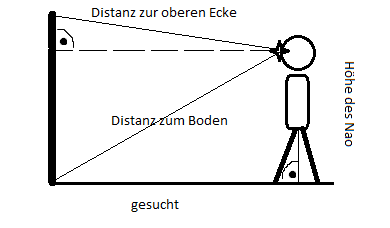
\includegraphics[scale=0.6]{Distanz_3D_Kugelkoordinaten_zu_2D_kartesisch}
\end{center}
\caption{Veranschaulichung des Problems}
\end{figure}
\begin{itemize}
\item Wir bekommen vom Server aller Objekte die wir sehen können als 
Kugelkoordinaten relativ zum Roboterkopf (bzw. zur Kamera). Im 
allgemeinen interessiert uns allerdings mehr die Distanz zwischen uns 
und dem Objekt. 
\item Glücklicherweise lässt sich das Problem einfach lösen: $\sqrt{(Distanz)^2 - (\texttt{Nao-Augenhoehe})^2}$
\item Problem: Bei manchen Objekten liefert uns der Server die Distanz
 und Winkel zur oberen Ecke (z.B. Goal). Das verkompliziert das Problem 
aber nur minimal:
\item $\sqrt{(Distanz)^2 - (\texttt{Objekthoehe} - \texttt{Nao-Augenhoehe})^2}$
\item \textbf{WICHTIG! Deshalb sollte man die Positionsbestimmung abschalten wenn man merkt das man umgefallen ist!}
\end{itemize}
\subsubsection{Eigene Position bestimmen}
\begin{figure}[h]
\begin{center}
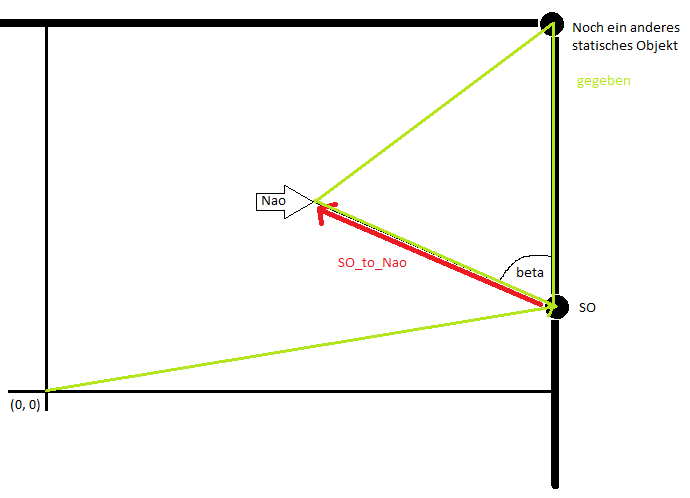
\includegraphics[scale=0.6]{Positionsbestimmung}
\end{center}
\caption{Skizze}
\end{figure}
\begin{figure}[h]
\begin{center}
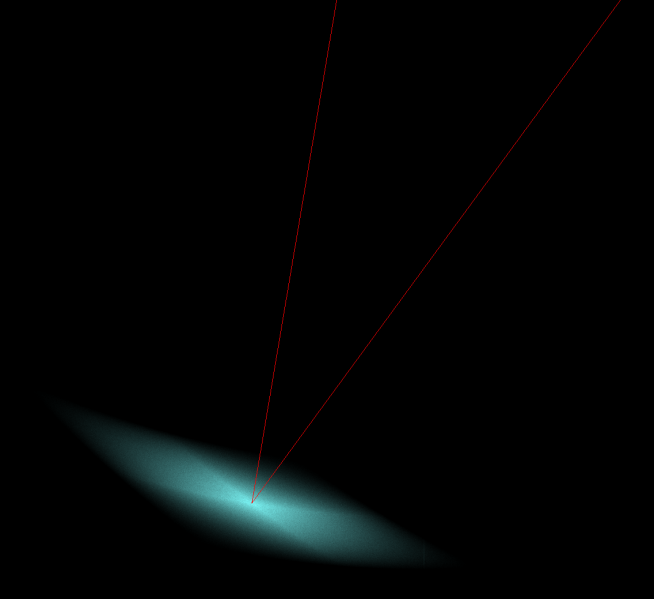
\includegraphics[scale=0.3]{654px-Pos_wahrscheinlichkeit}
\end{center}
\caption{Wahrscheinlichkeitsverteilung unserer ermittelten Position}
\end{figure}
\begin{itemize}
\item Was haben wir?
\begin{itemize}
	\item  Wir wissen wo sich die Flaggen, Linien und Torpfosten befinden.
 Bzw. anders formuliert wir kennen die Vektoren zu ihrer Position.
	\item  Wir bekommen vom Server die Distanz zu diesen Objekten (sofern wir sie denn sehen).
	\item  Damit haben wir dann zusammen mit der Distanz zwischen den 
statischen Objekten (die ist immer gleich und uns bekannt) ein hübsches 
Dreieck.
	\item   \textbf{ Wir brauchen immer min. 2 statische Objekte im Sichtfeld!}
\end{itemize}
\item  Was wollen wir?
\begin{itemize}
	\item  Den Vektor vom Koordinatenursprung zu unserer Eigenen Position.
\end{itemize}
\item  Wie bekommen wir den? 
\begin{itemize}
	\item  1. Berechne beta an SO (z.B. mit dem Kosinussatz für beliebige Dreiecke). (Siehe Skizze!)
	\item  2. Berechne ob SO das linke oder rechte Objekt ist.
	\begin{itemize}
		\item  Wir haben die Winkel zu den Objekten, von daher müssen wir 
testen welcher größer ist. (Im Sinne von mathematisch positiv bedeutet 
ein höherer Wert weiter links.)
	\end{itemize}
	\item  3. Berechne den Vektor von SO zu unserer eigenen Position. (In der Skizze SO\_to\_Nao)
	\begin{itemize}
		\item  Die Länge kennen wir ja schon, es fehlt nur noch die Richtung.
		\item  Nun drehen wir den den Vektor zwischen den statischen Objekten
 um unser beta *(-1) (im Uhrzeigersinn) wenn es das Linke ist und um 
beta (gegen den Uhrzeigersinn) wenn es das Rechte ist.
		\begin{itemize}
			\item  (Das ist total abgefahrene Mathemagie, weil man in das 
Koordinatensystem 2 Dreiecke malen kann die die entsprechende 
Seitenlängen haben und so auf 2 verschiedene Lösungen kommen könnte. Wir
 sparen uns also das Rätselraten das wir beim Berechnen der 
Schnittkreise haben.)
		\end{itemize}
		\item  Wir passen seine Länge auf unsere gegebene Distanz an.
	\end{itemize}
	\item  4. Der Finale Schritt
	\begin{itemize}
		\item  Addiere den Vektor aus 3. zu dem Vektor vom Koordinatenursprung zu SO und glelange endlich ans Ziel~:D
	\end{itemize}
\end{itemize}
\end{itemize}
\subsubsection{Mobile Entitäten lokalisieren}
\begin{itemize}
\item  Gesucht: absolute, kartesische Positionskoordinaten einer beweglichen Entität (\texttt{MobileEntity}, also \texttt{Ball} oder \texttt{Player})
\item  Gegeben:
\begin{itemize}
	\item  die Richtung, in die der NAO guckt als absoluten, kartesischen 3D-Vektor (\texttt{see\_vector})
	\item  eine Angabe in Polarkoordinaten, wo im Blickfeld des NAOs und wie weit entfernt sich die entsprechende Entität befindet (\texttt{pol})
\end{itemize}
\item  Lösung:
\begin{itemize}
	\item  Wir nehmen den \texttt{see\_vector} und:
	\begin{itemize}
		\item  berechnen aus dessen 2D-Teil (ohne z) einen Winkel \texttt{rot2d}
	\end{itemize}
	\item  Dann rotieren wir \texttt{see\_vector}:
	\begin{itemize}
		\item  um die z-Achse um \texttt{-rot2d} auf die xz-Ebene (so, dass y = 0)
		\item  um die y-Achse um den vertikalen Winkel in \texttt{pol}
		\item  um die z-Achse um den horizontalen Winkel in \texttt{pol} + \texttt{rot2d}
	\end{itemize}
	\item  Wir normieren den entstandenen Vektor.
	\item  Wir skalieren ihn um die Distanz in \texttt{pol} (Entfernung von Kamera zu Objekt).
	\item  Da isse, die mobile Entität.
	\end{itemize}
\end{itemize}
\subsubsection{Umgang mit Rauschen}
\begin{figure}[h]
\begin{center}
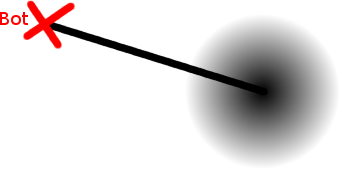
\includegraphics[scale=0.6]{MPGI3-RC-13S_Wahrscheinlichkeit2}
\end{center}
\caption{Vereinfachte Annahme: Rauschen kreisförmig verteilt}
\end{figure}
\begin{figure}[h]
\begin{center}
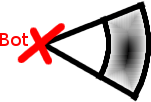
\includegraphics[scale=0.6]{MPGI3-RC-13S_Wahrscheinlichkeit1}
\end{center}
\caption{Tatsächliche Situation: Winkel- und Distanz-Rauschen}
\end{figure}
Um (später) die Genauigkeit unserer Positionsbestimmungen zu erhöhen,
 sollten wir beachten, welche Formen sich uns bei der Betrachtung der 
Wahrscheinlichkeitsverteilungen präsentieren.\\
Die einfachere Variante wäre, nach der Positionsbestimmung \textit{ein}
 einfaches Skalar mit abzuspeichern, das die ungefähre Genauigkeit der 
Position angibt. Diese lässt sich als Radius einer Kugel / eines Kreises
 (wenn wir auf 3D verzichten) interpretieren. (obere Abbildung)\\
Tatsächlich sieht die Verteilung aber eher so aus wie in der unteren Abbildung.

\paragraph{Einfache Positionsbetimmung über Schnittpunkte von Kreisen}
- Wird im Moment nicht verwendet! Sollte iegentlich zur 
Positionsbestimmung genutzt werden, wurde aber durch einen besseren 
Ansatz verdrängt.
Allerdings könnte es zur Berechnung der erwarteten Abweichung noch sehr 
nützlich sein, von daher erstmal behalten!

\begin{itemize}
\item  1. Wir definieren um 2 statische Objekte Kreise mit ihrer Position als Mittelpunkt und dem Abstand zum Agenten als Radius. 
\begin{itemize}
	\item  Z.B. $k = (x-x_M)^2 + (y-y_M)^2 - Distanz^2 = 0$
\end{itemize}
\item  2. Wir berechnen die beiden Schnittpunkte der Kreise.
\begin{itemize}
	\item  1.  $k_1 - k_2$
	\item  2. nach y umstellen ~~> eine Gerade c: m * x + n (die nennt man übrigens Chordale)
	\item  3. Setze c in die Kreisgleichung ein. ~~> 2 Ergebnisse
	\item  4. Setze die aufgelöste Variable in c ein und erhalte die beiden zugehörigen Koordinatenpaare.
\end{itemize}
\item  Um zu bestimmen an welche Position wir uns nun tatsächlich 
befinden würde ich vorschlagen das wir zu uns zu jedem Zeitpunkt merken 
ob wir im Spielfeld sind oder nicht. Da all unsere statischen Objekte am
 Spielfeldrand liegen wäre eine Position immer im und die andere 
außerhalb des Spielfeldes.
\begin{itemize}
	\item  Ist es möglich zu jedem Zeitpunkt zu wissen wo ob man im Spielfeld ist oder nicht?
\end{itemize}
\item  können wir uns vielleicht irgendwie berechnen in welche 
Richtung wir gerade schauen und dann überlegen welches der beiden 
Objekte links bzw. rechts ein müsste wenn wir im Spielfeld sind?
\item Wir könnten auch unsere zu letzt bekannte Position mit einbeziehen.
\begin{itemize}
	\item kann man ohne es zu wissen plötzlich außerhalb des Spielfelds landen?
\end{itemize}
\end{itemize}
\begin{itemize}
\item  Vorteile:
\begin{itemize}
	\item  sehr schnell
	\item  kommt ohne den Winkel phi aus -> man spart sich einen weiteren verrauschten Parameter
\end{itemize}
\end{itemize}
